\section{Basic concepts of linear algebra}
The following are the main concepts of linear algebra we are going to face during the starting phase of the course:
\begin{enumerate}
    \item Linear systems of equations: $A\underline{x} = \underline{b}$
    \item Eigenvalues and eigenvectors: $A\underline{x} = \lambda \underline{x}$
    \item Singular value decomposition (SVD):$A\underline{v} = \sigma u$
    \item Minimization problem
    \item Factorization: $PA = LU$
\end{enumerate}


% $\mathbb{A}\underline{x} = \lambda \underline{x}$
% $\mathbb{A}\underline{v} = \sigma \mathbb{u}$

\section{Matrix-vector multiplication}
\[
\underline{c} = \underbrace{\begin{bmatrix}
    1 & 2\\
    3 & 4\\
    5 & 6
\end{bmatrix}}_{A_1}
\underbrace{\begin{bmatrix}
    x_1\\
    x_2
\end{bmatrix}}_{\underline{x}}
= 
\begin{bmatrix}
    1x_1 + 2x_2\\
    3x_1 + 4x_2\\
    5x_1 + 6x_2 
\end{bmatrix}
=
\underbrace{
\begin{bmatrix}
    1\\
    2\\
    3
\end{bmatrix}
x_1+
\begin{bmatrix}
    4\\
    5\\
    6
\end{bmatrix}
x_2
}_{\text{linear combination}}
\]
We say that the vector $\underline{c}$ belongs to the \textbf{column space} of $A_1$, i.e. $\underline{c} \in \mathcal{C}(A_1)$.
\[
\overbrace{
\underbrace{
\begin{bmatrix}
    1 & 4 & 7\\
    2 & 5 & 8\\
    3 & 6 & 9
\end{bmatrix}}_{\underline{a_1} \hspace{0.2cm} \underline{a_2} \hspace{0.2cm} \underline{a_3}}
}^{A_2}
\begin{bmatrix}
    x_1\\
    x_2\\
    x_3
\end{bmatrix}
\]
In this case we can easily notice that $\underline{a_3} = \underline{a_1} + \underline{a_2}$, which means that one column can be expressed as a linear combination of the other two (this means that the matrix $A_2$ is singular). Because of this, we can say that $\mathcal{C}(A_2) = \mathcal{C}(A_1)$, i.e. the column space of $A_2$ is the same as the column space of $A_1$.

Those columns spaces are a plane passing through the origin and spanned by the two vectors $\underline{a_1}$ and $\underline{a_2}$ (they define the slope of that plane).

Let's now consider these matrix:
\[
\underbrace{
\begin{bmatrix}
    1 & 4 & 7\\
    2 & 5 & 8\\
    3 & 6 & 10
\end{bmatrix}
}_{A_3} 
\hspace{3cm}
\underbrace{
\begin{bmatrix}
    1 & 2 & 3\\
    2 & 4 & 6\\
    3 & 6 & 9
\end{bmatrix}
}_{A_4} 
\]
This left-hand matrix column space is $\mathcal{C}(A_3) = \mathbb{R}^3$, i.e. the entire real space of three dimensions. This is because the three vector columns of $A_3$ are linearly independet so they span the entire space and not just a plane.
While the column space of $A_4$ is instead: $\mathcal{C}(A_3) = \begin{bmatrix}
    1&2&3
\end{bmatrix}^T$ i.e. just a line since the three columns are linearly dependent and so they lie on the same line (they are parallel) just with different magnitude.

Another measure regarding matrices is the \textbf{dimension} or \textbf{rank}:
\begin{itemize}
    \item $rank(A_1) = 2$
    \item $rank(A_2) = 2$
    \item $rank(A_3) = 3$
    \item $rank(A_4) = 1$
\end{itemize}
The rank is the number of linearly independent columns (or rows) of a matrix.

Let's consider again the matrix $A_3$:
\[
\begin{bmatrix}
    1 & 4 & 7\\
    2 & 5 & 8\\
    3 & 6 & 10
\end{bmatrix}
\begin{bmatrix}
    x_1\\
    x_2\\
    x_3
\end{bmatrix}
= 
\underbrace{\begin{bmatrix}
    1\\
    2\\
    3
\end{bmatrix}
x_1+
\begin{bmatrix}
    4\\
    5\\
    6
\end{bmatrix}
x_2+
\begin{bmatrix}
    7\\
    8\\
    10
\end{bmatrix}
x_3}_{\in \mathcal{C}(A_3)}
=
\begin{bmatrix}
    b_1\\
    b_2\\
    b_3
\end{bmatrix}
\]
so $\underline{b}$ must be in $\mathcal{C}(A_3)$ in order to have the system solvable. If $\underline{b} \notin \mathcal{C}(A_3)$, then the system is not solvable. In this particular case we have that the columns of $A_3$ are linearly independent, so the system is solvable for any $\underline{b}$ because $\mathcal{C}(A_3) = \mathbb{R}^3$ and so $\underline{b}$ is for sure inside that space. \\

Given A, find $\mathcal{C}(A)$. How can we solve this problem? Considering $\underline{a_1}, \dots, \underline{a_n}$ as A columns, we can use the following iterative algorithm:
\begin{itemize}
    \item put $\underline{a_1}$ in $\mathcal{C}(A)$
    \item if $\underline{a_2} = \alpha \underline{a_1} \rightarrow \underline{a_2} \notin \mathcal{C}(A)$, otherwise put $\underline{a_2}$ in $\mathcal{C}(A)$
\end{itemize}
Until you reach the last column.

\subsection{Row-reduced echelon form}
Given the matrix $A$, defined as follow:
\[
A = \begin{bmatrix}
    1 & 4 & 7\\
    2 & 5 & 8\\
    3 & 6 & 9
\end{bmatrix}
\]
we can obtain the \textbf{row-reduced echelon form} of $A$ by applying the following operations:
\[
A = CR = \begin{bmatrix}
1 & 4\\
2 & 5\\
3 & 6
\end{bmatrix}
\begin{bmatrix}
    1 & 0 & -1\\
    0 & 1 & 2
\end{bmatrix}
\]
where $C$ is the matrix containing the columns of $A$ that are linearly independent (i.e. $\mathcal{C}(A)$) and $R$ is the matrix of the coefficients of the linear combination of the columns of $A$ that gives the columns of $C$.\\

Let's now consider the following matrix:
\[
A_1 = \begin{bmatrix}
1 & 4\\
2 & 5\\
3 & 6
\end{bmatrix}  
\hspace{2cm}
A_1^\intercal = \begin{bmatrix}
1 & 2 & 3\\
4 & 5 & 6
\end{bmatrix}  
\]
What we can say about $A_1^\intercal$ column space? Is there any relationship with the column space of $A_1$?

In order to compute its column space, we can start noticing that: $\underline{a_3} = 2\underline{a_2} - \underline{a_1}$. So, in general, we can say that:
\[
dim(\mathcal{C}(A)) = dim(\mathcal{C}(A^\intercal)) = r \leq n \hspace{1cm} \text{where $n$ is the number of columns of $A$}
\]

\section{Matrix-matrix multiplication}
\[
C = AB = \begin{bmatrix}
    \vline & \vline & \vline\\
    \underline{a_1} & \ldots & \underline{a_n}\\
    \vline & \vline & \vline
\end{bmatrix}
\begin{bmatrix}
    \horzbar & \underline{b_1} & \horzbar\\
    \horzbar & \vdots & \horzbar\\
    \horzbar & \underline{b_n} & \horzbar
\end{bmatrix}
= \overset{\overset{\text{col}}{\downarrow}}{\underline{a_1}}\overset{\overset{\text{row}}{\downarrow}}{\underline{b_1}} + \dots + \underline{a_n}\underline{b_n}
\] 
All the products that are summed at the end of the equation are matrices of rank 1. 

Example:
\[
\begin{bmatrix}
1 & 2\\
3 & 4
\end{bmatrix}  
\begin{bmatrix}
    2 & 1\\
    2 & 3
\end{bmatrix}
= \underbrace{
    \begin{bmatrix}
        2 & 1\\
        6 & 3
    \end{bmatrix}
}_{\text{rank = 1}}
+ \underbrace{
    \begin{bmatrix}
        4 & 6\\
        8 & 12
    \end{bmatrix}
}_{\text{rank = 1}}
= \begin{bmatrix}
    6 & 7\\
    14 & 15
\end{bmatrix}
\]


\section{Factorizations}
\begin{enumerate}
    \item $A = LU$ or $PA = LU$
    \item $A = QR$ where $Q$ is orthogonal and $R$ is upper triangular
    This is an improved version of the Row-reduced echelon form because that worked only for square matrices, while this works for any matrix.
    \item Eigenvalues and eigenvectors decomposition: when $S = S^\intercal$ (symmetric matrix) we can factorize it as $S = Q\Lambda Q^\intercal$ where $\Lambda$ is a diagonal matrix and $Q$ is an orthogonal matrix (they are all squared matrices)
    \item Generalization of the above: $A = X\Lambda X^{-1}$ where $X$ is a non-orthogonal matrix
    \item $A = U\Sigma V^\intercal$ where $U$ and $V$ are orthogonal matrices and $\Sigma$ is a pseudo-diagonal matrix
\end{enumerate}
A matrix is said to be pseudo-diagonal if it has the following form:
\[
    \Sigma = 
    \begin{bmatrix}
        \sigma_1 & 0 & 0 & 0\\
        0 & \sigma_2 & 0 & 0\\
        0 & 0 & \ddots & 0\\
        0 & 0 & 0 & \sigma_n\\
        0 & 0 & 0 & 0\\
        \vdots & \vdots & \vdots & \vdots\\
        0 & 0 & 0 & 0
    \end{bmatrix}
    \hspace{2cm}
    m \text{ rows} \times n \text{ columns}
\]
So it has diagonal elements for the first $n$ rows then it has all zeros.

\subsection{Orthogonal matrices}
A matrix $Q$ is orthogonal if $Q^\intercal Q = I$ (i.e. $Q^\intercal = Q^{-1}$). This means that the columns of $Q$ are orthonormal, i.e. they are orthogonal and have unit norm.\\

The determinant of a orthogonal matrix is $\pm 1$.

Properties:
\begin{itemize}
    \item $||Q\underline{x}|| = ||\underline{x}||$
    \item $||Q\underline{x}||^2 = (Q\underline{x})^\intercal Q\underline{x} = \underline{x}^\intercal \underbrace{Q^\intercal Q}_{I} \underline{x} = ||\underline{x}||^2$
\end{itemize}
The first property is particularly easy to interpret since it means that when we multiply an orthogonal matrix to a vector, the norm of the vector doesn't change. As a proof of this, we can consider the following examples:

\subsubsection{Rotation}
A classical rotation matrix is:
\[
\begin{bmatrix}
    cos(\theta) & -sin(\theta)\\
    sin(\theta) & cos(\theta)
\end{bmatrix}    
\]
\subsubsection{Reflection}
\begin{center}
    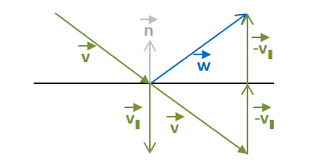
\includegraphics[scale=0.5]{../images/Reflection.png}
\end{center}
The horizontal line in the figure represent a plane $\pi$ while $\underline{n}$ is its normal vector of length 1. 
Given $\underline{v}$ to obtain $\underline{w}$ we can use the following formula:
\[
\underline{w} = \underline{v} - 2(\underline{v}^\intercal \underline{n})\underline{n} = \underbrace{(I - 2\underline{n}\underline{n}^\intercal)}_{\text{reflection matrix}}\underline{v}
\]
Moreover, the reflection matrix $R$ is not only orthogonal, but also the inverse of itself, i.e. $R^{-1} = R^\intercal$. This makes sense because if we apply the reflection matrix twice, we obtain the original vector $\underline{v}$, i.e. the reflection of the reflection is the starting vector.

If we didn't have the 2 in the formula, we would obtain the projection of $\underline{v}$ on the plane $\pi$ which is called orthogonal projection and the matrix $R$ would be singular. \\

Let's now dive a bit into the third point of the factorization list. We said that when $S = S^\intercal$ (symmetric matrix) we can factorize it as $S = Q\Lambda Q^\intercal$ where $\Lambda$ is a diagonal matrix and $Q$ is an orthogonal matrix.\\
\[
S = S^\intercal = \underbrace{(Q\Lambda))}_{\tilde{Q}}Q^\intercal = \tilde{Q}Q^\intercal   
\]
\[
\tilde{Q} = \underline{q_1}\underline{\lambda_1} + \dots + \underline{q_n}\underline{\lambda_n}    
\]
Where the $q$ vectors are columns and $\lambda$ vectors are rows.
So we can reformulate:
\[
    S = (\underline{q_1}\underline{\lambda_1} + \dots + \underline{q_n}\underline{\lambda_n})Q^\intercal = \underline{q_1}\underline{\lambda_1}\underline{q_1}^\intercal + \dots + \underline{q_n}\underline{\lambda_n}\underline{q_n}^\intercal
\]
This is called \textbf{spectral decomposition} of matrix $S$ and $q_1, \dots, q_n$ are the eigenvectors of $S$ while $\lambda_1, \dots, \lambda_n$ are the eigenvalues of $S$.
\[
    S\underline{q_1} = \lambda_1\underline{q_1} = (\underline{q_1}\underline{\lambda_1}\underline{q_1}^\intercal + \dots + \underline{q_n}\underline{\lambda_n}\underline{q_n}^\intercal)\underline{q_1} = 
    \underline{\lambda_1}\underline{q_1}(\underline{q_1^\intercal}\underline{q_1})
    \]
All the other products are null since the vector $\underline{q_1}$ is orthogonal to all the other vectors $\underline{q_i}$ for $i \neq 1$ (recall that they are eigenvectors).

\section{Null spaces}
Let's consider the starting problem for a linear system of equations:
\[
A\underline{x} = \underline{b} \hspace{1cm} \text{with} \hspace{1cm} A\in \mathbb{R}^{m \times n}, \text{rank($A$)}=r    
\]

We are going to introduce 2 more spaces other than the column ones. To do so we consider:
\[
  A\underline{x} = \underline{0} \hspace{1cm} \rightarrow \hspace{1cm} N(A) \equiv \ker(A) = \{\underline{x} \in \mathbb{R}^n : A\underline{x} = \underline{0}\}  
\]
\[
    A^\intercal\underline{x} = \underline{0} \hspace{1cm} \rightarrow \hspace{1cm} N(A^\intercal) \equiv \ker(A^\intercal) = \{\underline{x} \in \mathbb{R}^n : A^\intercal\underline{x} = \underline{0}\}    
\]

So now, adding the so called \textbf{null spaces} we have that:
\begin{enumerate}
    \item $\mathcal{C}(A) \subset  \mathbb{R}^m$ and $dim(\mathcal{C}(A)) = r$
    \item $\mathcal{C}(A^\intercal) \subset \mathbb{R}^n$ and $dim(\mathcal{C}(A^\intercal)) = r$
    \item $N(A) \subset \mathbb{R}^n$ and $dim(N(A)) = ?$
    \item $N(A^\intercal) \subset \mathbb{R}^m$ and $dim(N(A^\intercal)) = ?$
\end{enumerate}
We still do not know the dimensions of those spaces. \\

\textbf{Example}\\
\[
A = \begin{bmatrix}
    1 & 4 & 7\\
    2 & 5 & 8\\
    3 & 6 & 9
\end{bmatrix}
\begin{bmatrix}
    x_1\\
    x_2\\
    x_3
\end{bmatrix}
= 
\begin{bmatrix}
    0\\
    0\\
    0
\end{bmatrix}
\hspace{0.3cm} \implies \hspace{0.3cm}
\begin{cases}
    x_1 + 4x_2 + 7x_3 = 0\\
    2x_1 + 5x_2 + 8x_3 = 0\\
    3x_1 + 6x_2 + 9x_3 = 0
\end{cases}    
\]
We compute the first equation
\[
    x_1 = -4x_2 - 7x_3 \hspace{0.3cm} \implies \hspace{0.3cm} \begin{cases}
        -3x_2 - 6x_3 = 0\\
        -6x_2 - 12x_3 = 0
    \end{cases}
\]
What is important to notice is that $A$ has rank$=2$ so we have $3-2=1$  \textbf{degrees of freedom}, i.e. we can choose one variable and the other two are automatically defined. This is visible in the last two equations of the system for example. 
In general, the degrees of freedom are given by $n-r$ where $n$ is the number of columns of $A$ and $r$ is the rank of $A$.\\

If we had 10 instead of 9 in $A$ we would have had $3-3=0$ degrees of freedom. This would translate in having the matrix $A$ full rank and $N(A) = \{\underline{0}\}$ so the only solution would be the null vector.

